% !TeX spellcheck = en_GB

\section{DSS To DWH}

\begin{breakbox}
\boxtitle{Grouping Sets:}
\sql{sql_code/grouping_sets.sql}
With the \lstinline{GROUPING(column)} command it is possible
to see if this value is grouped.
\sql{sql_code/grouping_command.sql}
\end{breakbox}

\begin{breakbox}
\boxtitle{SUM over partitions:}
\sql{sql_code/multiple_sums.sql}
\end{breakbox}

\begin{breakbox}
\boxtitle{LAG/LEAD:}
\sql{sql_code/lag.sql}
Instead of  \lstinline{LAG(n)} \lstinline{LEAD(n)} can be used to get n records
in advance.
\end{breakbox}

\begin{breakbox}
\boxtitle{RANK:}
\sql{sql_code/rank.sql}
\end{breakbox}

\begin{breakbox}
\boxtitle{AVG and formatting:}
\sql{sql_code/avg_format.sql}
To get following cells the \lstinline{FOLLOWING} keyword is used instead of
\lstinline{PRECEEDING}.
\end{breakbox}

%\begin{breakbox}
%\boxtitle{Analytische Aggregatoren:}
%\begin{center}
%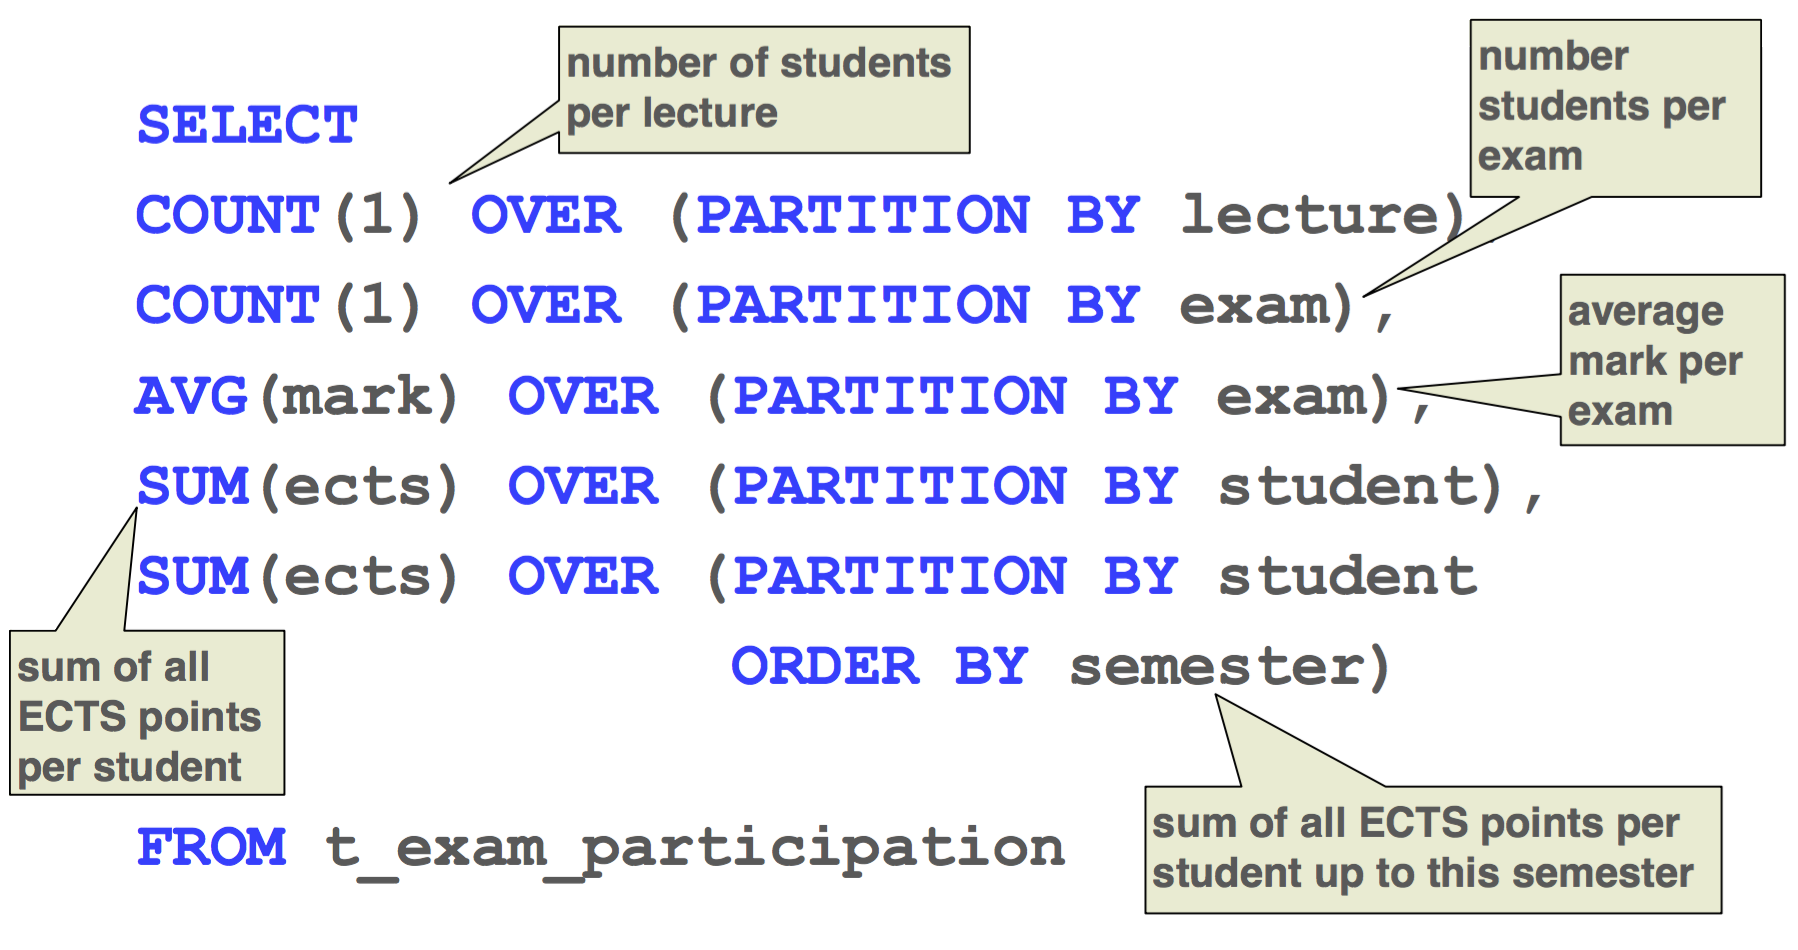
\includegraphics[width=.12\textwidth]{slides_images/analytical_aggregate_functions}
%\end{center}
%\end{breakbox}

\begin{breakbox}
\boxtitle{Additional analytical functions:}
\begin{itemize}
	\item VAR\_POP(), VAR\_SAMP(), STDDEV\_POP(), STDDEV\_SAMP()
	\begin{itemize}
		\item determine variance and standard dviation
	\end{itemize}
	\item RANK(), DENSERANK()
	\begin{itemize}
		\item establish a ranking, with or without gaps
	\end{itemize}
	\item FIRST\_VALUE(), LAST\_VALUE()
	\begin{itemize}
		\item gives first (last) value of a sort sequence
	\end{itemize}
	\item CORR()
	\begin{itemize}
		\item calculate correlation
	\end{itemize}
	\item RATIO\_TO\_REPORT()
	\begin{itemize}
		\item value's proportion of total of partition
	\end{itemize}
	\item NTILE()
	\begin{itemize}
		\item divides each partition in n like fractions (quarters, tenths, halves etc.)
	\end{itemize}
\end{itemize}	
\end{breakbox}

\begin{breakbox}
\boxtitle{OLTP vs. OLAP:}
OLTP are the working databases where all the applications write into
(different) databases. In OLAP all the operational databases are integrated
into one DB for \textbf{analytical processes.}
\begin{itemize}
	\item Workload:
	\begin{itemize}
		\item OLTP: predictable / constantly high
		\item OLAP: unpredictable / erratic
	\end{itemize}
	\item Units of work / Transactions:
	\begin{itemize}
		\item OLTP: small / often writing
		\item OLAP: large, only reading
	\end{itemize}
	\item Performance / Requirements:
	\begin{itemize}
		\item OLTP: strict
		\item OLAP: varying
	\end{itemize}
	\item Queries:
	\begin{itemize}
		\item OLTP: simply structured
		\item OLAP: complex
	\end{itemize}
\end{itemize}
\end{breakbox}
